\subsection{Spectral Clustering}
\label{subsec:spectralclusteringresults}

\begin{figure}[ht!]
    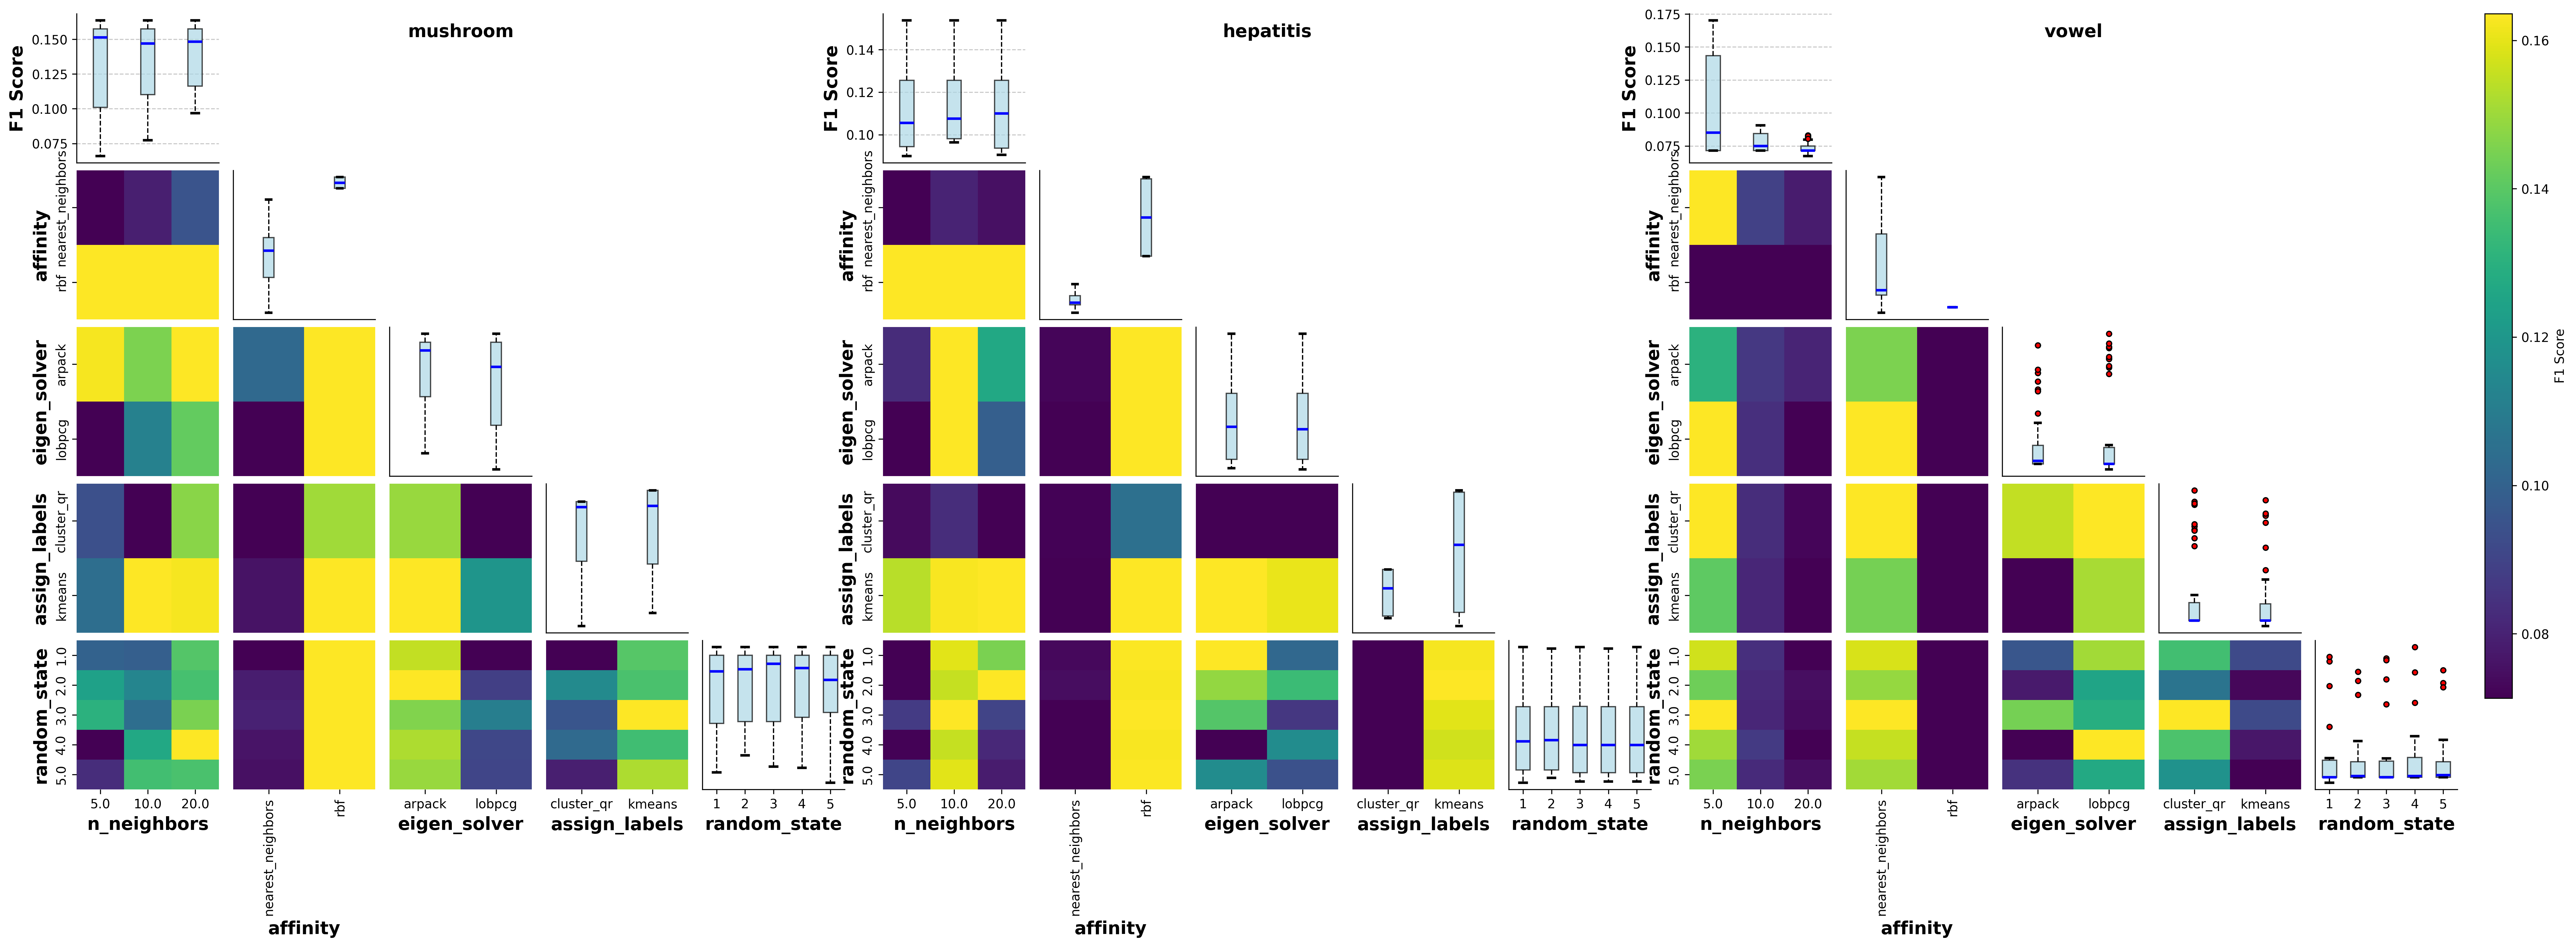
\includegraphics[width=0.5\textwidth]{figures/interactions_spectral_clustering.png}
    \caption{Parameter interactions for Spectral Clustering}
    \label{fig:interactions_spectral}
\end{figure}

As seen in \ref{fig:interactions_spectral}, spectral clustering showed varying performance across different parameter configurations and datasets. It achieved roughly 0.15 F1 scores at best across the datasets, including achieving an F1 of 0.16 on the mushroom dataset using RBF affinity with ARPACK solver and assigning labels using kmeans. It was the best performing method on the difficult-to-cluster vowel dataset, with an F1 score of 0.17.

The algorithm's performance was significantly influenced by several key parameters:

\begin{itemize}
    \item \textbf{Affinity Matrix}: Nearest-neighbors consistently outperformed RBF kernel for the vowel dataset, while RBF showed superior results for the mushroom and hepatitis datasets
    \item \textbf{Solver Choice}: LOBPCG solver generally provided faster execution times (0.03-0.08s) compared to ARPACK (0.1-0.4s), and the results were similar
    \item \textbf{Number of Neighbors}: Lower values (n\_neighbors=5) produced more stable results for the vowel dataset, but it mattered less for the other datasets
    \item \textbf{Assignment Method}: cluster\_qr and kmeans assignments showed similar clustering quality
    \item \textbf{Random State}: The results were very similar across different random states, indicating that the results are consistent and not highly dependent on the initialization
\end{itemize}

We saw interesting interactions between the parameters. For example, using a Kmeans assignment with the rbf affinity matrix showed particular effectiveness on the hepatitis dataset.
